\documentclass[fleqn,10pt]{wlscirep}
\usepackage[utf8]{inputenc}
\usepackage[T1]{fontenc}
\usepackage{float}
\usepackage{indentfirst}
\usepackage{booktabs}  % Để kẻ dòng kẻ đẹp (toprule, midrule)
\usepackage{graphicx}  % Để dùng resizebox co giãn bảng
\usepackage{array}     % Để xử lý căn chỉnh cột
\usepackage{float}     % Để dùng [H] cố định vị trí
\title{DEEP LEARNING FOR SKIN LESION SEGMENTATION: A REVIEW}

\author[]{Duy Hung BUI 202412987}
\author[]{Huy Hoang VU 202412982}

%\keywords{Keyword1, Keyword2, Keyword3}

\begin{abstract}

    Computer-Aided Diagnosis (CAD) systemes for melanoma require accurate skin lesion segmentation. Over the past decade, Deep Learning (DL) models have become the standard for this problem; howerver, in order to solve artifacts and fuzzy boundaries, there must be sophisticated optimizing strategies. This review shows a comprehensive look to computational techniques, which are categorized by their optimizing objectives. Firstly, we discuss the foundational Convolutional Neural Network (CNN) developments, from structural improvement models including Improved U-Net, Fully Convolutional Network (FCN)-based U-Net, and receptive field expansion models such as Deeplab, to automated hyperparameter management with Bayesian SegNet and attention mechanism integration models like Attention Gates, CBAMSNet. Secondly, we analyze the change to global context model FAT-Net utilising Hybrid Transformers solving the disadvantage of local inductive tendency of CNNs. Finally, we evaluate the new trend of 2024: Mamba. For instance, hybrid models such as AC-MambaSeg and VM-SwimUNet have shown their capability of balancing segmentation accuracy and linear computational efficiency ($O(N)$). The review also highlights the role of Generative Adversarial Networks (GANs) in data augmentation, which provides a perspective for developing next-generation clinical diagnostic systems.

\end{abstract}
\begin{document}

\flushbottom
\maketitle
% * <john.hammersley@gmail.com> 2015-02-09T12:07:31.197Z:
%
%  Click the title above to edit the author information and abstract
%
\thispagestyle{empty}
\section*{Introduction}
    
    The skin plays a vital role as an interface between the human body and the environment, governing essential functions such as the body temperature regulation and fluid retention. In spite of the resilience, the skin is prone to a multitude of pathologies. It is estimated that there are over 3,000 distinct types of dermatological disorders, which makes skin diseases one of the most challenging health concerns worldwide. Global Cancer Statistics 2020 states that annually, fatal skin lesions claim thousands of lives \cite{GlobalCancer}. More precisely, skin cancer ranks as the third most common human malignancy, with melanoma being its most aggressive and lethal form. Epidemiological data indicates a rapid surge in melanoma incidence over the last three decades. Notably, statistical projections estimated approximately 96,480 new diagnoses in the United States in 2019 \cite{Melanoma}.

    Dermoscopy, a non-invasive imaging technique, has improved the accuracy; however, manual interpretation of dermoscopic images is labor-intensive, subjective, and dependending heavily on the clinician's expertise. Therefore, CAD systems turn out to be indispensable tools in clinical dermatology. Within the CAD pipeline, skin lesion segmentation, which is the process of accurately delineating the lesion boundary from the surrounding healthy skin, is the most critical prerequisite.
    
    Accurate recognition of melanoma is regarded as challenges due to multiple of complexities. To begin with, the low contrast between lesions and the surrounding healthy skin often creates ambiguous boundaries \cite{FCN, GAN, Deeplab}.  Secondly, high variability in patient-specific attributes, ranging from skin pigmentation and texture to lesion morphology, complicates the detection process \cite{UNet, GAN, Deeplab, Transformer}. Furthermore, image usually contains various artifacts, including body hair, reflections, air bubbles, shadows, and inconsistent illuminating conditions \cite{FCN, UNet, GAN,Transformer}. Thirdly, the scarcity of training data leads to a severe constraint on the model's generalization capability. Fourthly, the class imbalance problem, where the lesion area is smaller than the background, significantly deters segmentation performance. Notably, these aforementioned occlusions and artifacts are pervasive in standard public dermoscopic datasets. Figure 1 visually exemplifies these impediments, showing the complexity in precise boundary delineation.

        \begin{figure}[H]
        \centering
        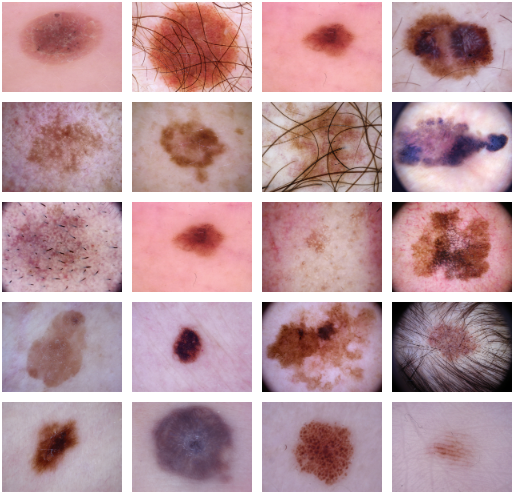
\includegraphics[width=0.6\linewidth]{ISIC2018.png}
        \caption{Dermoscopic images of some of the skin diseases from the ISIC 2016 dataset \cite{Skin}.}
        \label{fig:skindiseases}
        \end{figure}

    Early DL approaches such as FCN and U-Net, established a strong baseline but they would be struggled when there was a complex lesion heterogeneity. Consequently, recent research has moved beyond "vanilla" architectures, putting efforts on optimizing foundational models. For example, integrating structural designs (Improved U-Net), automating hyperparameter tuning (Bayesian SegNet), and evaluating attention mechanisms (Attention Gates, CBAMSNet) to enhance feature selection. Despite these solutions, CNN-based methods still remain limitation from their local receptive fields, failing to capture long-range semantic dependencies effectively.

    So as to shorten the gap, Vision Transformers (ViTs) and its hybrid models like FAT-Net were introduced, leveraging self-attention to model global context. However, quadratic computational complexity ($O(N^2)$) of ViTs has resulted in a barrier to deploy on low resource clinical devices. This trade-off has catalyzed the emergence of Mamba in 2024, offering not only the global modeling capability of Transformers but also the linear efficiency ($O(N)$) of CNNs.

    In this paper, we categorize each approach based on their optimization strategies: from data augmentation by Generative Adversarial Networks (GANs) and structural optimizations of CNNs, to the global context modeling of Transformers, and finally, the efficiency-driven era of Mamba models such as AC-MambaSeg, VM-SwinUnet. Our aim through this analysis is to identify the directions for future real-time diagnostic systems. To visualize this landscape, \textbf{Fig. \ref{fig:taxonomy}} presents the taxonomy of the computational techniques reviewed in this study.
        
        \begin{figure}[H]
            \centering
            \includegraphics[width=0.65\linewidth]{Taxonomy.jpg}
            \caption{Taxonomy of computational techniques for skin lesion segmentation utilized in this survey, categorizing methods from foundational CNNs to hybrid Mamba models.}
            \label{fig:taxonomy}
        \end{figure}

\section*{The Computational Pipeline \& Data Preparation}
    The quality of training data plays a decisive role in the performance of DL models that obey to the fundamental principle of "Garbage In, Garbage Out." particularly in dermatological analysis, the presence of artifacts and severe class imbalance necessitates sophisticated computational strategies before segmentation.

    \subsection*{Artifact Removal and Normalization}
        Artifacts such as body hair, gel bubbles, ruler markers, and uneven illumination in dermoscopic images may prevent lesion boundaries and mislead feature extraction. To deal with these issues, multiple standard pre-processing pipelines are introduced to normalize the training data. 

        Artifact Removal: Hair occlusion is the most common impediment. The DullRazor algorithm is among the standard computational approaches for the task, identifying dark hair structures using generalized grayscale morphological closing operations and subsequently replacing the occluded pixels with values interpolated from the surrounding non-occluded tissue.

        Color Normalization: Dermoscopic images are taken under different conditions of lights, color inconsistency by a wide variety of devices, preventing model convergence. Techniques such as Shades of Gray or Gray World algorithms are used to standardize the illumination and normalize the color distribution. Such methods adjust the color channels based on the average intensity, ensuring that the skin tones are consistent across the dataset.

    \subsection*{Advanced Data Augmentation Strategy via GANs}

        Class imbalance and lack of data diversity are noticing challenges in training robust skin lesion segmentation models, especially for malignant melanoma, which is always minor in public datasets. Traditional augmentation techniques, such as geometric transformations (rotation, flipping) and color jittering, are widely applied to increase the dataset size. However, these methods only produce variations of existing samples and fail to introduce sufficient diversity into the data distribution. To address the limitation, GAN has been employed as advanced data augmentation strategy. To be more precise, a GAN model consists of two competing neural networks: a Generator ($G$) and a Discriminator ($D$). $G$ tries to combine realistic lesion images from random noise distributions, while $D$ works as a binary classifier, distinguishing between real images and the synthetic ones produced by $G$. Through a min-max adversarial training process, $G$ will learn to produce excellent lesion samples capturing the complex texture and color characteristics of real dermoscopic images, which can consideralbly widen the training data.

            \begin{figure}[H]
            \centering
            \includegraphics[width=0.85\linewidth]{GAN.jpg}
            \caption{The flowchart of Dual Discriminator GAN architecture. After the generator module, there are two discrimination branches. One uses the concatenation of the generated mask and the original image as input, the integration is performed along the channel. The other just employs the generated mask as input.}
            \label{fig:GAN}
            \end{figure}

        Dual Discriminators by Lei et al. \cite{GAN} is an example of succeeded adversarial learning in leveraging segmentation, using $G$ for segmentation, and two distinct $D$ to supervise the results as \textbf{Fig. \ref{fig:GAN}}:

            \begin{itemize}
                \item A Global $D$ ensures the overall structural consistency of the predicted mask.
                \item A Local $D$ concentrates more on the boundary details, especially the lesion edges.
            \end{itemize}

        The system of "double scrutiny" can learns to generate not only pixel-wise accurate but also visually consistent segmentation. This study has shown the versatile potential of GANs: acting as both a tool for data augmentation and a segmentation mechanism through adversarial loss.

    \section*{Optimizing Foundational CNN Architectures}

        While early CNNs marked a noticeable change from manual feature extraction to automated learning, vanilla models often struggle with the specific challenges of dermoscopy, such as fuzzy boundaries and low contrast. Hence, the first era of advancement was defined not merely by the application of CNNs, but by the rigorous optimization of foundational architectures. This section categorizes these computational improvements into three strategic domains: structural improvement, receptive field expansion, and attention-based feature selection.

    \subsection*{Structural and Hyperparameter Optimization}

        The transition from patch-based classification to pixel-wise segmentation was pioneered by FCNs. However, the approach usually suffered from resolution loss during upsampling. To solve this, a author \cite{FCN} proposed a FCN-based model optimized with a U-Net-like architecture as \textbf{Fig. \ref{fig: FCN}}. By adapting the FCN to learn end-to-end mappings while incorporating symmetric decoding paths, the model is capable of minimizing the loss of spatial information, demonstrating that FCNs can be structurally managed to deal with quality lesion details.

            \begin{figure}[H]
                \centering
                \includegraphics[width=0.85\linewidth]{FCN.jpg}
                \caption{The flowchart of U-Net like architecture bases on FCN model.}
                \label{fig:FCN}
            \end{figure}

        Another method is to optimize the training hyperparameters. The SegNet architecture, known for its memory-efficient utilising pooling indices, is highly sensitive to parameter initialization. Sahin et al. \cite{SegNet} introduced a Bayesian Optimized SegNet which replaces manual trial-and-error by Bayesian probability. Compared with standard SegNet implementations, the model achieved superior segmentation accuracy by automatically searching for the optimal learning rate compared to standard SegNet implementations. This approach has proved that in training process, it is vital to optimize not only the architectural designs but also the computational methods.

    \subsection*{Expanding Receptive Fields via Dilated Convolutions}
            
        Standard U-Net model can be overfitting with small datasets, and limited by fixed receptive field. Liu et al. \cite{UNet} proposed an Improved U-Net \textbf{Fig. \ref{fig: UNet}} applying dialated convolution and batch normalization layer in the decoder to expand the receptive field. Therefore, the encoder-decoder path can preserve the edge information and cut down on false positives due to coarse boundary compared to the classic U-Net.

        \begin{figure}[H]
            \centering
            \includegraphics[width=0.85\linewidth]{UNet.jpg}
            \caption{The flowchart of Improved U-Net model with dialated convolution and batch normalization.}
            \label{fig:UNet}
        \end{figure}


        The author \cite{Deeplab} introduced a hybrid model between RetinaNet and DeepLab incorporating a Graph-based refinement algorithm for post-processing. The RetinaNet backbone is responsible for extracting multi-scale features, while the DeepLab module employs atrous spatial pyramid pooling (ASPP) to capture context at multiple scales. The graph-based refinement step further enhances boundary accuracy by modeling pixel relationships as a graph, allowing for more precise delineation of lesion edges. By combining the object detection strength of RetinaNet, the semantic context of DeepLab, and the boundary precision of graph theory, the method overcomes the local view limitation of standard CNNs.

    \subsection*{Feature Selection with Attention and Dynamic Mechanisms}

        As network depth increases, the risk of learning redundant features (e.g., background artifacts like hair or gel) rises. To enable the network to "focus" on relevant regions, Attention Mechanisms were introduced.

        Arora et al. \cite{AttentionGates} integrated Attention Gates (AGs) into the U-Net architecture. Unlike hard attention which crops images, AGs employ soft attention to automatically learn weight coefficients that suppress irrelevant background regions while highlighting feature-rich lesion areas. This mechanism allows the model to inherently filter out artifacts without explicit pre-processing.

        Pushing the envelope of optimization further, recent works like CBAMSNet \cite{CBAMSNet} have combined attention with dynamic computation. This architecture integrates the Convolutional Block Attention Module (CBAM) to refine features along both channel and spatial dimensions. More importantly, it employs Omni-dimensional Dynamic Convolution (ODConv), where convolutional kernels are not static but dynamically adapt their weights based on the input image. This "dynamic" capability allows the network to be lightweight and computationally efficient while maintaining the flexibility to handle the high variability of skin lesion shapes.

\section*{The Shift to Global Context with Hybrid Transformers}

    While the optimized CNN architectures discussed in the previous section significantly improved boundary delineation, they remain bound by the inherent limitation of the convolution operation: the local receptive field. Even with dilated convolutions (as in DeepLab), CNNs struggle to capture long-range dependencies explicitly. In complex dermatological cases, where the diagnosis depends on the relationship between widely separated visual patterns, this local inductive bias becomes a bottleneck.

    To address this, the second era of computational techniques is defined by the integration of Transformers, leveraging the Self-Attention mechanism to model global context.

    \subsection*{Hybrid Architecture Strategy: The FAT-Net Case}

        Pure Transformers (like the original ViT) often suffer from localized feature loss due to patch partitioning and require massive datasets to converge. Therefore, the dominant strategy in medical imaging is the Hybrid Approach.

        A prime example is FAT-Net (Feature Adaptive Transformers) proposed by Wu et al. \cite{Transformer}. Instead of discarding the CNN entirely, FAT-Net employs a Dual-Encoder Strategy: 
        
            \begin{itemize} 
                \item A ResNet-50 backbone is used to extract high-resolution spatial features. 
                \item Transformer layers are embedded at the bottleneck to capture global semantic relationships.
            \end{itemize}

        The core computational innovation of FAT-Net is the Feature Adaptive Module (FAM). Recognizing that skin lesions often possess irregular shapes and varying sizes, the FAM utilizes channel attention to adaptively activate relevant feature maps while suppressing noise. Furthermore, to mitigate the high memory consumption typically associated with Transformers, the authors designed a Memory-Efficient Decoder. This structural optimization allows FAT-Net to achieve a superior Dice score compared to U-Net and Att-Unet, proving that combining the "local detail" of CNNs with the "global vision" of Transformers is more effective than using either in isolation.
\section*{The Efficiency Revolution with State Space Models (Mamba)}
    Despite the success of Hybrid Transformers, they come with a significant computational cost: the self-attention mechanism scales quadratically with image size ($O(N^2)$). This complexity renders them challenging to deploy on resource-constrained devices, such as mobile dermoscopy systems. In 2024, a paradigm shift occurred with the emergence of State Space Models (SSMs), specifically the Mamba architecture, which offers the global modeling capability of Transformers with linear computational complexity ($O(N)$).
        \subsection*{The Adaptive Hybrid (AC-MambaSeg)}
            Representing the fusion of CNN flexibility and Mamba efficiency, AC-MambaSeg \cite{Mamba} serves as a state-of-the-art benchmark. \textbf{Nguyen et al.} replaced the heavy convolutional backbone with Visual State Space (VSS) blocks. These blocks utilize a 2D Selective Scan (SS2D) mechanism to flatten the image into sequences and scan them in four directions, capturing global context without the quadratic cost of attention matrices.Crucially, AC-MambaSeg does not abandon the optimizations of the past. It integrates Attention Gates (from Era 1) in the skip connections and utilizes Selective Kernel (SK) modules to adaptively adjust the receptive field size. By synergizing the linear speed of Mamba with the feature-focusing capability of legacy attention mechanisms, AC-MambaSeg achieves a balance between high inference speed and segmentation accuracy.
        \subsection*{The Ultimate Fusion (VM-SwinUnet)}
            While AC-MambaSeg targets efficiency, VM-SwinUnet represents the pursuit of maximum accuracy through a "Super-Hybrid" design. This architecture combines Swin Transformer blocks with VSS (Mamba) blocks.The computational rationale here is complementary: Swin Transformers excel at extracting hierarchical features via shifted windows (local-to-global), while Mamba blocks model long-range dependencies across the entire image (global). This fusion mitigates the "local forgetting" problem of pure Mamba models and the heavy computational load of pure Transformers. Although more complex, VM-SwinUnet demonstrates that for critical diagnostic tasks where accuracy is paramount, integrating the strengths of CNNs, Transformers, and SSMs into a unified framework yields the best performance metrics.
\section*{Discussion \& Comparative Analysis}
    The evolution from foundational CNNs to modern Mamba architectures illustrates a clear trajectory in computational optimization.
    \begin{table}[H]
        \centering
        \caption{Comparative Analysis of Computational Paradigms in Skin Lesion Segmentation based on Optimization Strategies.}
        \label{tab:comparison}
        \resizebox{\textwidth}{!}{%
        \begin{tabular}{l l l p{4cm} l}
        \toprule
        \textbf{Paradigm} & \textbf{Model} & \textbf{Core Mechanism} & \textbf{Key Strength} & \textbf{Complexity} \\ 
        \midrule
        \textbf{Optimized CNN} & Improved U-Net & Structural Refinement & Precise Boundary Delineation & Low $\mathcal{O}(N)$ \\ 
        & DeepLab & Atrous Convolution & Expanded Receptive Field & Low $\mathcal{O}(N)$ \\ 
        \midrule
        \textbf{Attention CNN} & Attention U-Net & Soft Attention Gates & Artifact Suppression (Hair/Gel) & Low $\mathcal{O}(N)$ \\ 
        & CBAMSNet & ODConv + CBAM & Dynamic Feature Adaptation & Low $\mathcal{O}(N)$ \\ 
        \midrule
        \textbf{Hybrid Transformer} & FAT-Net & Self-Attention + FAM & Global Context Modeling & High $\mathcal{O}(N^2)$ \\ 
        \midrule
        \textbf{Hybrid Mamba} & AC-MambaSeg & VSS Block (Selective Scan) & Global Context with Linear Speed & \textbf{Linear $\mathcal{O}(N)$} \\ 
        & VM-SwinUnet & Mamba + Swin Trans. & High-Performance Fusion & Moderate \\ 
        \bottomrule
        \end{tabular}%
        }
    \end{table}
    
\section*{Conclusion}
    This review has traversed the landscape of computational techniques for skin lesion segmentation, categorizing them by their optimization objectives rather than mere chronology. We analyzed how GANs address data scarcity, how Optimized CNNs (e.g., FCN, DeepLab) refined structural and contextual learning, and how Transformers (FAT-Net) bridged the global context gap. Finally, we highlighted the 2024 breakthrough of Mamba architectures (AC-MambaSeg, VM-SwinUnet), which achieve linear complexity without compromising accuracy. We conclude that the future of automated melanoma diagnosis lies in Hybrid Systems—architectures that leverage the speed of Mamba, the precision of Transformers, and the localized focus of attention mechanisms to deliver real-time, clinically reliable diagnoses.
\section*{Methods}

Topical subheadings are allowed. Authors must ensure that their Methods section includes adequate experimental and characterization data \cite{FCN}necessary for others in the field to reproduce their work.

\bibliography{sample}

\end{document}